% !TEX root = AImath.v4.tex
\chapter{语言中的智能：Transformer的意外胜利 \texorpdfstring{\\}{ }让机器“听懂”世界的第一步？}

%\chapter{生成式AI：机器魔法}
 \begin{introduction}
  \item Transformer架构的革命性突破
  \item 注意力机制的数学原理与实现
  \item 大语言模型的涌现能力分析
  \item 从序列到序列的智能转换
  \item 语言理解与生成的数学建模
\end{introduction}

“山中方七日，世上几千年”

“动荡时代的最大风险不是动荡本身， 而是企图以昨天的逻辑来应对动荡
The greatest danger in times of turbulence is not the turbulence; it is to act with yesterday’s logic.”
\begin{flushright}
— 彼得·德鲁克 Peter F. Drucker
\end{flushright}


“【生成式AI】大模型+大资料=神奇结果？”

近年来，生成模型在人工智能领域取得了显著的进展，特别是在图像生成方面。从简单的图像生成到复杂的文本到图像转换，生成模型展现了强大的潜力和广泛的应用前景。生成对抗网络(GANs)和变分自编码器(VAEs)等传统方法虽然取得了成功，但仍面临一些挑战，如训练不稳定性和生成质量的限制。因此，研究人员不断探索新的方法来提升生成模型的性能。

%本文将介绍一种先进的生成模型---StableDiffusion，该模型在文本到图像生成任务中表现出色，通过扩散过程实现高质量图像的生成。

\begin{figure}[htbp]
\centering
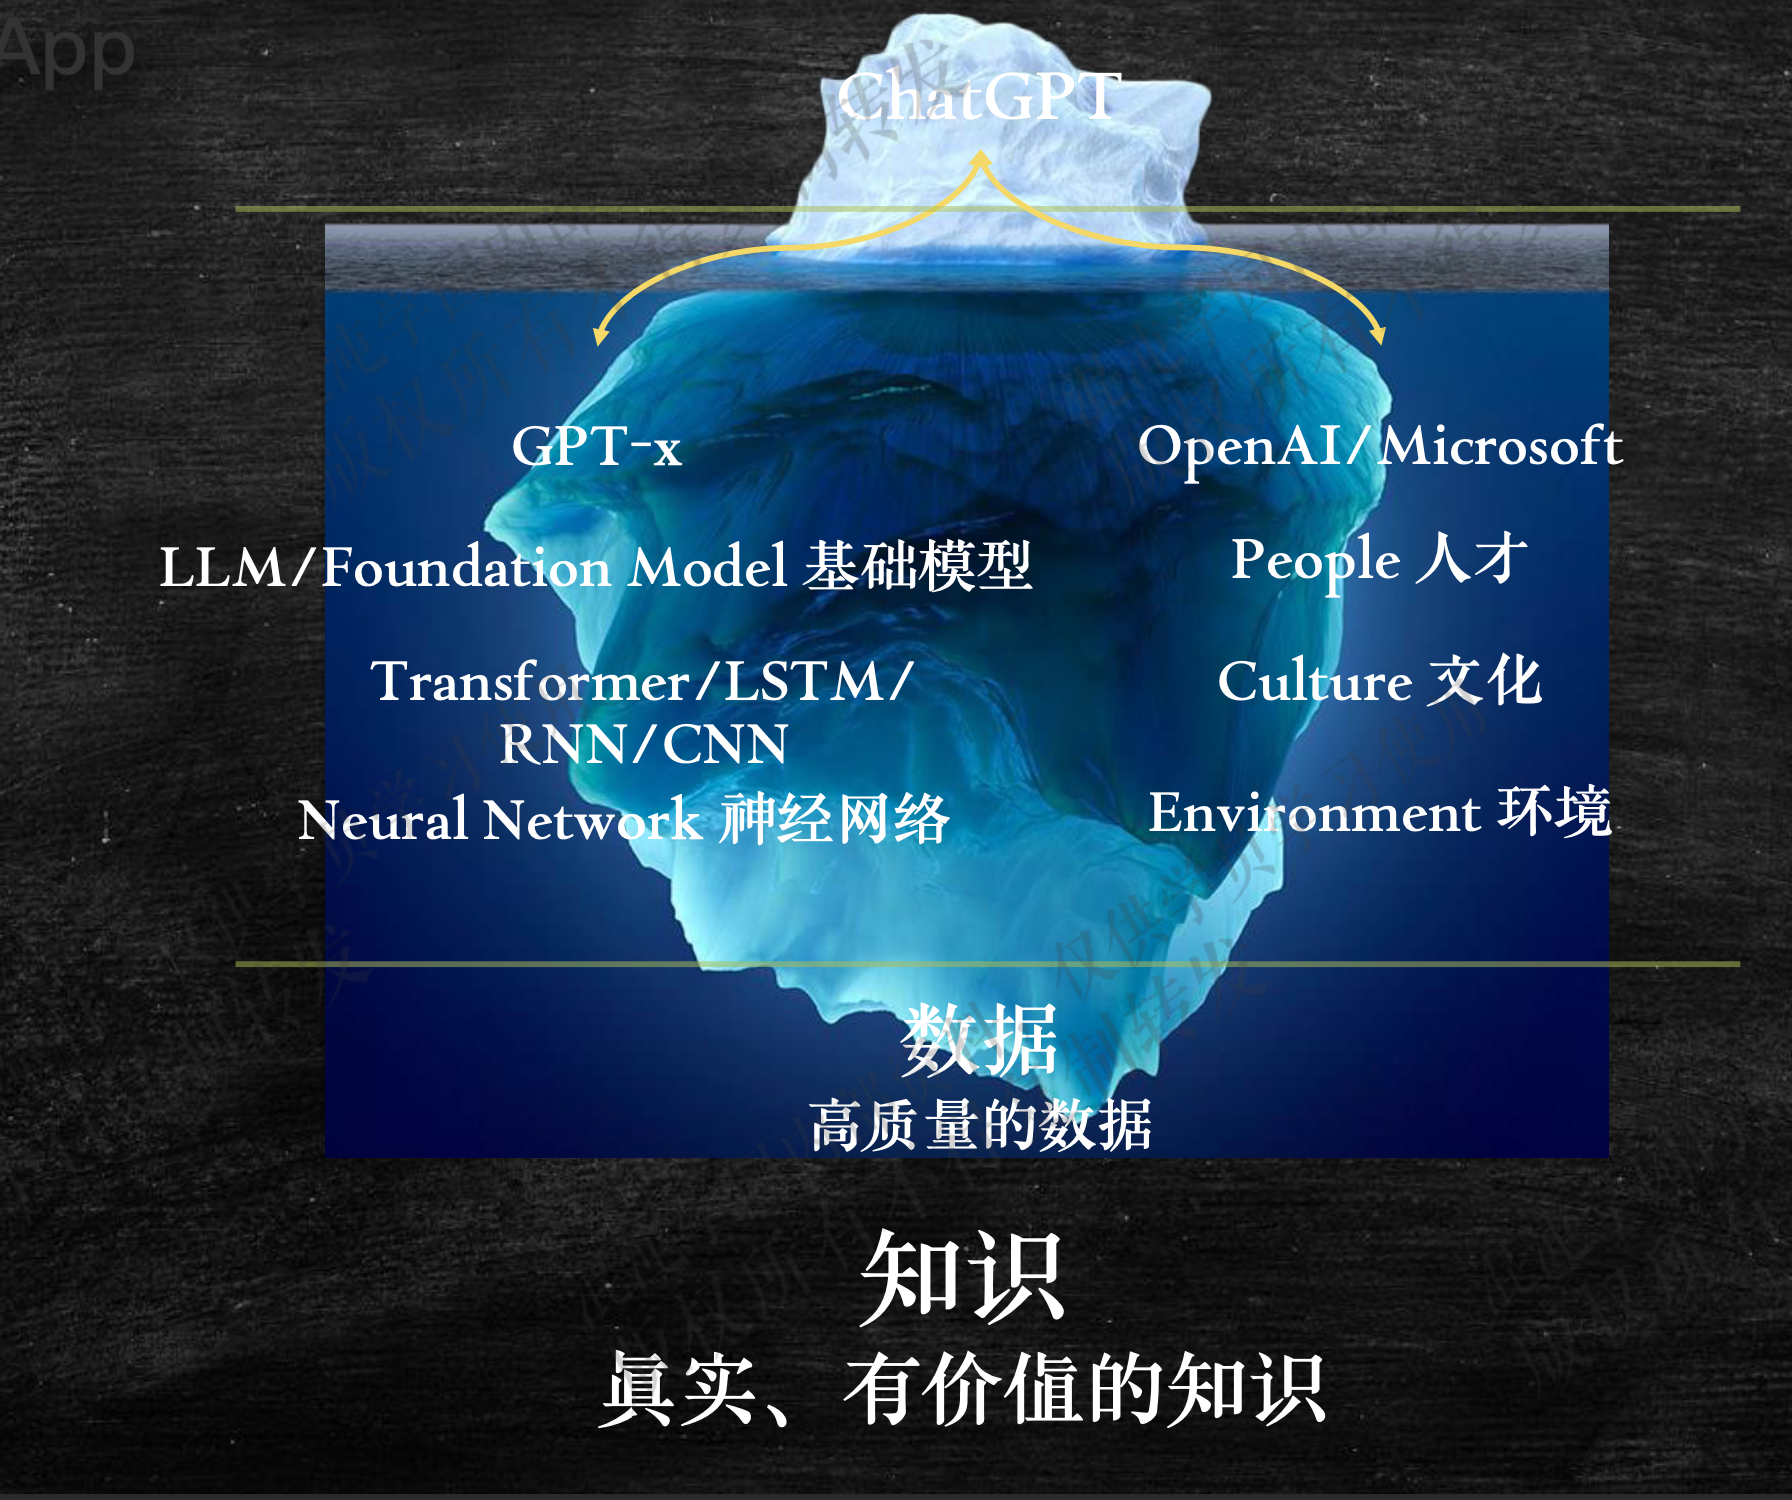
\includegraphics[width=0.3\textwidth]{figs/冰山.png}
\caption{“ChatGPT冰山下的”}
%\label{}
\end{figure}



%\section{背景}
生成模型是人工智能中的重要研究方向，旨在生成逼真的图像、文本和其他数据。传统方法如生成对抗网络(GANs)和变分自编码器(VAEs)在图像生成中取得了显著成果，但它们也存在一些局限性。例如，GANs的训练过程通常不稳定，容易出现模式崩溃(ModeCollapse);而VAEs生成的图像质量往往不够高。为了解决这些问题，StableDiffusion引入了基于扩散过程的新方法，通过模拟数据的随机演化行为，从而实现高效且稳定的图像生成。StableDiffusion利用扩散过程的优点，在生成质量和稳定性方面取得了显著进展。


%\section{什么是Stable Diffusion}
StableDiffusion是一种基于Latent Diffusion Models(LDMs)的生成模型，专为文本到图像生成任务设计。其核心思想是通过扩散过程，从随机噪声逐步生成符合文本描述的高质量图像。StableDiffusion利用扩散过程模拟数据的随机演化行为，确保生成过程的稳定性和高效性。模型首先从随机噪声开始，经过一系列的变换和调整，逐步接近目标图像。这一过程可以理解为在潜在空间中的变换，使得生成的图像能够准确反映输入的文本描述。Stable Diffusion的独特之处在于其双向扩散机制:正向扩散将文本描述转化为潜在表示，反向扩散则从潜在表示生成最终图像。

%\section{核心原理}

StableDiffusion的核心原理包括两个主要阶段:
扩散过程:模型从随机噪声开始，逐步应用一系列变换，使其逐渐接近目标图像。这一过程模拟了数据的随机演化行为，确保生成过程的稳定性和高效性。在扩散过程中，模型学习到数据的分布特性，并利用这些特性对噪声进行调整。
反向扩散过程:与扩散过程相反，反向扩散是将噪声逐步变换为目标图像的过程。在这一过程中，模型根据学习到的数据分布特性，逐步去噪并生成符合文本描述的图像。反向扩散过程利用参数化的马尔可夫链进行建模，通过逐步调整和优化，最终生成高质量的图像。
通过这两个阶段的有机结合，StableDiffusion能够高效地将文本描述转化为高质量的图像，展示出强大的生成能力和应用前景。

%\section{应用场景}
StableDiffusion在多个领域中有广泛应用，包括但不限于:

-艺术创作:通过将文本描述转化为图像，艺术家可以利用StableDiffusion进行创作，探索新的艺术形式和风格。

-广告设计:广告设计师可以使用StableDiffusion根据客户需求生成定制的广告图像，提高设计效率和创意表现力。

-虚拟现实:在虚拟现实应用中，StableDiffusion可以根据文本描述生成逼真的虚拟场景，提升用户体验。

-医疗图像处理:在医疗领域，StableDiffusion可以根据医生的描述生成医学图像，辅助诊断和治疗。

这些应用展示了StableDiffusion在图像生成领域的广阔前景和巨大潜力，为各行各业提供了新的工具和方法。


%生成式对抗网络
%如果你在纸上画了几只猫，那么哪一只更像“真正”的猫呢?你要怎么做才能量化你的涂鸦和真正的猫之间的相似性?怎么定义图像之间相似度的度量?
%这些问题的用处并非只局限在“你画我猜”（pictionary)游戏中。测定文字、声音和图像等复杂对象之间的相似性2已经成为实用贝叶斯主义者发起的最困难的挑战之一。这是因为，真正有趣的数据实际上都是这种复杂的对象，比如拉普拉斯的著作、心电图以及显微镜下缓步动物的图像。
%2或者更进一步，也可以考虑文字、声音、图像上的概率分布。
%我们以宇宙学为例。今天，这个领域的数据基本上就是天空在各种波长下的照片，从无线电波开始，跨越微波、红外线、可见光、紫外线、X射线，一直到射线。让天体物理学家深深着迷的问题，就是在给定天空的照片的情况下，得出不同宇宙学模型的可信参数。这就是贝叶斯公式的典型应用!
%这个计算对于纯粹贝叶斯主义者来说易如反掌，但对实用贝叶斯主义者来说却难于登天。与通常的情况一样，分母太长难以计算。但问题不止于此。因为宇宙学模型都非常复杂，即使是思想实验项需要的计算时间也会超出现实的限制。实际上，正因为这些模型属于贝叶斯网络3，所以它们在构建时就考虑到了模拟计算的可行性。也就是说，在合理的时间内，我们可以做的就是在宇宙学模型参数为的假设下，描绘模型中可能出现的图像。这就是所谓的生成模型4。
%3我们会在第17章再提到这一点。
%
%4换种说法，生成模型就是一组图像之类的复杂集合上的概率分布，但它只能通过模型仿真来研究。再换种说法，生成模型就是被设计成用于取样的模型。我们会在第17章进行更深入的讨论。
%因此，实用贝叶斯主义者必须依靠某些方法来绕过对思想实验项的直接计算。人们也将其称为无似然方法(likelihood-freemethod)。这种方法有很多变种，比如近似贝叶斯计算(Approximate Bayesian Computation，简称ABC)和带参数贝叶斯间接似然度(parametric Bayesian Indirect Likelihood，简称pBIL)。但自从2014年伊恩·古德费洛及其合作者发表的工作[18]以来，一种特殊的无似然方法似乎赢得了大量研究者在实用上的置信度，那就是生成式对抗网络(简称GAN)。
%直观来说，GAN的想法就是将玩“你画我猜”的人类玩家换成一个算法，它被称为“对抗者”或“教师”。这位“对抗者”的任务就是衡量模型生成的图像与真正的图像有多相似。为此，我们先抛一枚硬币，如果正面向上，那么我们就在庞大的真实图像库中抽选一张图像，否则要求模型生成一张图像。然后，无论图像来自哪里，我们都要求“对抗者”计算出它是真实图像的贝叶斯置信度。如果模型正确的话，从直觉上来说“对抗者”应该会混淆两种可能性，也就是会向任何提交的图像都赋予的概率。
%重点在于，为了让“对抗者”乐于给出自身的贝叶斯置信度，古德费洛等人提出，在图像为真实图像的情况下，“对抗者”需要付出的代价，反之则需要付出的代价。也就是说，我们以符合KL散度的方式来计算分数。
%此外，生成模型 subsequent also 尝试调整参数，使得生成的数据更接近真实数据。而关键在于，这一点有着明确的意义:无论输入真实的图像，还是模型生成的图像，生成的数据需要使“对抗者”给出的数值尽量靠近。实际上，用于衡量“对抗者”的贝叶斯置信度偏差的同一个分数也可以用来衡量模型的表现5!
%5所以模型和“对抗者”实际进行的是零和博弈!

%当我写下这段话的时候，GAN风头正劲。其惊人效果正不断得到提升，这主要得益于深度学习。2018年，GAN中的模型和“对抗者”实际上都换成了(卷积)神经网络6。正因它们能够对贝叶斯公式进行无似然近似，再加上神经网络学习的常用工具，GAN获得了巨大的能力，足以生成极其难以与真实照片区分的假照片[19]。从各个角度来说，正是概率性预测的新度量方法的出现才造就了这些现代人工智能激动人心的表现。
%一般来说，模型就是一个深度神经网络，再加上一个用于生成变量的“简单”概率分布。对模型进行模拟就会输出数据。“对抗者”是另一个深度神经网络。这种结构的好处就在于能够应用反向传播算法。这个算法能确定为什么选择了，然后将这项信息倒推回去，用以改进生成模型。在这种意义上，更像是“教师”，而不是“对抗者”。
%此外，为了给本章做个总结，我想再一次强调在判断预测质量的方法中考虑不确定性的重要性。不幸的是，在分析各种现象时，人们往往低估随机的作用。我们必须习惯在思考中考虑不确定性，而不是在那些本质上不可预测的情境中也要尝试做出确定性的预测。在这个复杂的宇宙中，没有任何认识是确定无误的，无论原因是现实的物理本质、经验数据的欠缺、混沌现象的存在，还是我们在计算能力上的限制。
%绝大部分预测问题没有简单一致的回答，回答这类问题时要谨慎。只有最终承认大量事件发生的原因都是运气不好，这种谨慎才站得住脚。因此，对模型与预测的判断必须能量化不确定性。量化不确定性实在非常重要，这件事不能被随意决定。
%
%
%人工智能的创新艺术
%人工智能学会作曲和绘画还是不久之前的事情。我们在第16章也简略提到过，这种创造性过程的关键还是贝叶斯公式。
%原因在于，在众多深度学习模型中，我们可以在神经网络中激活某些所谓的深度神经元，由此创造出抽象概念之间的结合体。其中一些神经网络就此能够想象出哪些原始数据能激活那些被人为激活的神经元。也就是说，虽然神经网络通常从数据推断出能够概括这些数据的抽象概念，但我们可以要求这些神经网络在已知抽象概念的情况下猜测可能与之有关的数据。
%然后，选择那些一般而言没有联系的抽象概念，我们就能让神经网络创造出一些既不常见但又相对可信的数据。这就是机器的艺术生成过程。我们可以打赌，这种过程至少与我们大脑中的创造性过程有几分相似。
%在2015年，谷歌利用这种方法，在研究博客上发表了人工智能“深梦”(DeepDream)生成的一些图像[1]。这些图像有种迷幻的感觉，人们在其中能看到云朵变成了鱼，树变成了寺庙，而树的叶子则变成了飞鸟。更妙的是，你可以要求另一个被称为“深艺”(DeepArt)的人工智能用著名画家的笔触重新诠释你拍的照片，无论是凡·高、毕加索还是康定斯基都可以。我的Twitter头像就是“深艺”花了几秒生成的免费劳动成果。
%在这些人工智能的创造性过程中，重要步骤之一就是神经网络在给定了数据的抽象概括的情况下，找到可信数据的能力。也就是说，神经网络应该能够根据数据|抽象概括这一概率分布，即给定被激活的抽象概念时数据出现的概率，进行抽样。这样的话，根据贝叶斯主义，创造性可以归结为根据带有语境的置信度进行抽样。
%但重要的是，抽样意味着给出有代表性的例子，而不是根据非常复杂的概率分布进行推理。在阐明推理并将其变得更易理解的过程中，这也许相当有用，毕竟哪怕是在数学中，人类的自然学习方式也似乎更倾向于依赖那些有代表性的例子，而不是形式化的理论。我们大脑中的设备似乎优化的是从例子中推断粗略规则的能力，而不是使神经网络符合形式化理论的能力。这就解释了为什么抽样对于人类来说不可或缺。古怪的是，抽样对于机器来说似乎同样不可或缺。
%但在讨论这一点之前，我们必须先找到合适的模型来表示数据与抽象概括之间的关系。人们提出了几种机器学习架构，用于描述概率分布以及根据这些分布进行抽样。这些结构可以分为两类(不同的复杂模型可以适当地结合在一起):贝叶斯网络(Bayesian network)--1它也被称为前馈模型(forward model)和马尔可夫随机场(Markov random field)。我们先来看看贝叶斯网络。
%
%
%隐含狄利克雷分布
%除了卡尔曼滤波器和隐马尔可夫模型，贝叶斯网络的主要成就之一就是在2000年前后提出的隐含狄利克雷分布(latent Dirichletal location，简称LDA)。LDA的目标是将文档分为不同的类别。计算机可以利用LDA以完全自动化的方式将你的电子邮件分别放到名为“私人”“工作”“度假”和“垃圾邮件”的文件夹中。更进一步的话，LDA even能检测出不同类别的组合，而且能判断某份文档的内容一半与工作有关，一半与度假有关，甚至判断出2/3属于私人内容，1/3属于工作内容。
%要做到这一点，LDA利用了贝叶斯网络中的基础概念，也就是因果性的概念，它的好处在于符合我们的直觉，这也使贝叶斯网络成了相对易于解释的概率模型。正是得益于贝叶斯网络与直觉之间的契合，尼尔和伯杰才提出可以在司法领域使用贝叶斯网络，就像我们在第2章中看到的那样。
文生文、文生图、文生视频



%篇幅约3900字（打印为5–6页），包括从语言的本质问题出发，回顾了NLP发展历程、Transformer的核心机制及其成功逻辑，并引发对“语言是否真的被理解”的深入思辨。本章是“回归与超越”的第一节，既呼应前文对建构方式的讨论，又为最后一章“理性与取舍的未来”埋下引子。

人类之所以被称为"智人"，部分原因在于我们拥有复杂的语言能力。而AI真正"破圈"的一次跃迁，不是让机器看懂猫，而是让它学会了说话---这背后，Transformer 是关键的结构性创新。

本章不试图教你如何实现一个Transformer模型，而是引导你理解：为什么它会在语言上"突然成功"？它的核心机制---自注意力（Self-Attention）---如何突破了过去模型对"顺序"的执念，又是如何实现了"全局关联"的理解？

结构提要：

Transformer 与传统 RNN/Seq2Seq 的关键差异

Self-Attention 的核心思想

为什么在语言上特别有效？

从BERT到GPT：语言世界的征服之路

结构设计的胜利，而非更深层"理解"


\section*{语言：智能最复杂的边疆}

在过去的章节中，我们从深度学习的困境出发，沿着图灵与哥德尔的理论边界，走过符号、神经与因果三种认知模式，也初步接触到智能的物理基础。

现在，让我们回到一个最贴近日常、也最神秘的智能领域：\textbf{语言}。

语言不仅仅是交流工具。它是人类思想的镜子，是知识的容器，是文化的脉络。一个真正的智能体，必须"理解"语言---而非仅仅模仿它。

但让机器理解语言，这也许是人工智能最古老、最难的问题之一。

直到近年，Transformer 架构的出现才带来某种“意外的胜利”：它没有使用语法规则、知识图谱或语言逻辑，而只是通过海量数据与注意力机制，就生成了看似“理解”语言的模型。

这是真正的理解，还是统计的幻觉？我们将在本章深入探讨。

\section*{语言建模的三座高墙}

自然语言处理（NLP）一直是AI中的“认知炼金术”，而它之所以难，源于三大核心挑战：

\begin{itemize}
\item \textbf{模糊性}（Ambiguity）：一个词可以有多种含义（如“银行”），一个句子可能有多种解释；
\item \textbf{上下文依赖}（Context Sensitivity）：意义往往依赖上下文甚至世界知识；
\item \textbf{长距离依赖}（Long-range Dependency）：语言中的相关成分可能间隔较远，例如主语和谓语之间插入多层修饰语。
\end{itemize}

早期方法试图用符号逻辑解决这些问题，比如基于句法树和形式语义学的系统；后来转向统计语言模型（如n-gram）尝试用概率建模，但总是力不从心。

直到 2017 年，Transformer 的提出彻底改变了NLP的进展曲线。

\section*{Transformer：自注意力的奇迹}

Transformer 的核心，是一种被称为“自注意力机制”（Self-Attention）的结构。

简单来说，自注意力机制可以让一个词在处理自身时，主动“关注”句子中的其他词，并按相关性赋予权重。

例如，在句子：
\begin{center}
\texttt{The trophy doesn't fit in the suitcase because \textbf{it} is too large.}
\end{center}
人类自然知道 “it” 指的是 “trophy” 而不是 “suitcase”。传统模型很难处理这种依赖，但 Transformer 能通过注意力权重“动态建立联系”，模拟出这种指代关系。

Transformer 还有几个关键特点：

\begin{itemize}
\item \textbf{并行性好}：与RNN不同，它不需要按顺序处理；
\item \textbf{捕捉长依赖}：即使句子很长，也能全局建模；
\item \textbf{架构通用}：从文本生成到多模态理解都能适用；
\item \textbf{层级结构}：多层注意力叠加，具备抽象表达能力。
\end{itemize}

从BERT到GPT，从T5到ChatGPT，Transformer 像一把“语言万用钥匙”，解锁了长期被压抑的建模能力。

\section*{语言生成的幻觉：理解，还是伪装？}

Transformer 的输出令人惊艳，但它真的“理解”语言了吗？

有人这样描述GPT的能力：“它预测下一个词，就像我们预测一个会说话的鹦鹉。”它能模仿人类，但是是否具备理解的内在机制？

这引出了几个深刻的的问题：

\begin{itemize}
\item 它能讲一个笑话---但它自己笑了吗？
\item 它能解释一个哲学观点---但它是否知道什么是"观点"？
\item 它能说"我明白"---但它是否真的"明白"？
\end{itemize}

许多研究指出：当前大型语言模型只是“惊人的词语压缩器”（stochastic parrots），它在庞大的语料中学会了生成“合理”但未必“真实”的语言。

比如：
- 它可以生成不存在的书籍引用；
- 它可以编造科学理论；
- 它可以逻辑自洽但事实错误。

这种现象揭示出一个本质悖论：\textbf{语言的可预测性≠语言的可理解性}。

\section*{知识、常识与推理的缺席}

语言模型真正缺乏的，不是词汇量，而是\textbf{对世界的结构性理解}。

- 它不知道“杯子不能放进瓶子里”的物理常识；
- 它无法稳定区分“因果”与“相关”；
- 它对时序、身份、空间等基本认知常常混乱。

这类缺陷通常通过如下方式被暴露：
- 对抽象问题的推理（如“如果火车晚点，我会错过会议吗？”）；
- 对多轮对话的一致性判断；
- 对“反事实问题”的应对（如“如果我昨天没去机场，现在会在哪？”）。

有人称之为"常识盲点"。这正是当前 Transformer 架构的局限---它只基于表层文本，而非深层知识图谱或因果模型。

\section*{神经–符号融合的语言建模尝试}

为了解决上述问题，研究者近年来尝试将语言模型与符号系统结合，形成“神经–符号语言智能”。

代表性尝试包括：

\begin{itemize}
\item \textbf{Neural Logic Machines}：将语言理解任务嵌入可微分的逻辑推理结构；
\item \textbf{Commonsense Transformers}：在预训练阶段引入常识知识库（如 ConceptNet）；
\item \textbf{RAG（Retrieval-Augmented Generation）}：结合检索系统与语言生成，强化外部知识；
\item \textbf{ChatGPT Plugin 架构}：通过工具调用增强模型对知识、代码、计算的外部访问。
\end{itemize}

这些方法都试图在语言建模中嵌入“知识调用”“工具使用”“因果判断”等能力，但融合仍处于初步阶段。

语言模型仍然强在“语感”而弱在“语义”。

\section*{语言的意义，是生成，还是参与？}

哲学家维特根斯坦曾说：“语言的意义，在于其使用。”这提醒我们，语言不是静态的知识库，而是一种社会行为、一种游戏、一种行为参与。

那么，当前的语言模型，是“参与者”还是“模仿者”？

它可以对话，但不能提出问题；
它可以总结，但不具备好奇；
它可以模仿表达，但未必有“立场”。

这让我们反思：\textbf{语言之智能，不只是生成能力，更在于交流意图、社会背景与情感共鸣}。

真正的"理解语言"，可能意味着对"人"的理解---这是目前AI尚难企及的地带。

\section*{下一章：理解之后，我们如何选择？}

Transformer 是一场奇迹，也是一面镜子。它展示了神经网络的潜力，也暴露了统计主义的局限。

下一章，我们将不再追问“AI是否足够聪明”，而是追问：“我们希望AI成为怎样的存在？”

这是关于伦理、责任与选择的议题。

这是理性之后，人类社会真正的试炼。

\nocite{*}
\printbibliography[heading=bibintoc, title=\ebibname]


\newpage


